\documentclass{article}
\usepackage{geometry}
\usepackage{graphicx}
\usepackage{amsmath}
\usepackage{algorithm}
\usepackage{algpseudocode}

\geometry{
a4paper,
right=20mm,
left=20mm,
top=20mm,
bottom=20mm,	
}

\begin{document}

\pagenumbering{gobble}

\begin{center}
\textbf{\Large Theoretical Assignment 6 : CS345} \\
\textit{\large Jayant Agrawal}         14282 \\
\textit{\large Shubham Pandey}         14679
\end{center}

\section{An Atmospheric Science Experiment}

\subsection{Part 1}
\begin{figure}[h!]
\centering
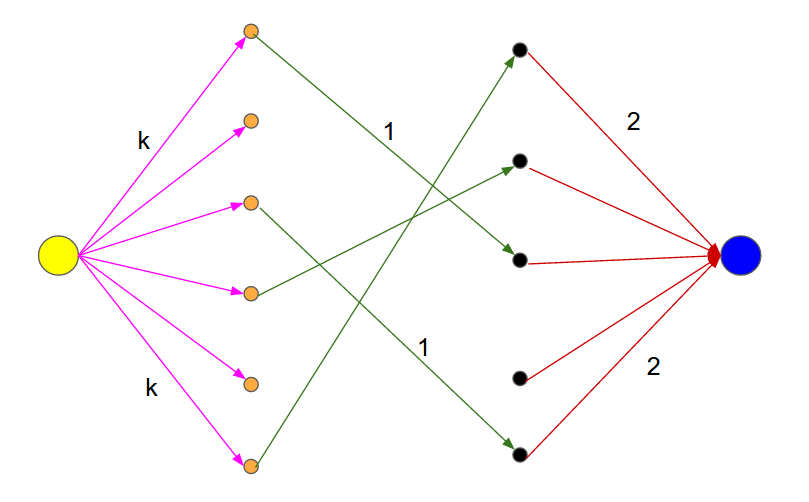
\includegraphics[width=0.5\columnwidth]{fig_one.png}
\caption{ Edge Capacities-- Pink Edges: k, Green Edges: 1, Red Edges: 2;\newline Orange Vertices: Conditions; Black Vertices: Balloons}
\label{sim}
\end{figure}

\subsection{Part 2}
\begin{figure}[h!]
\centering
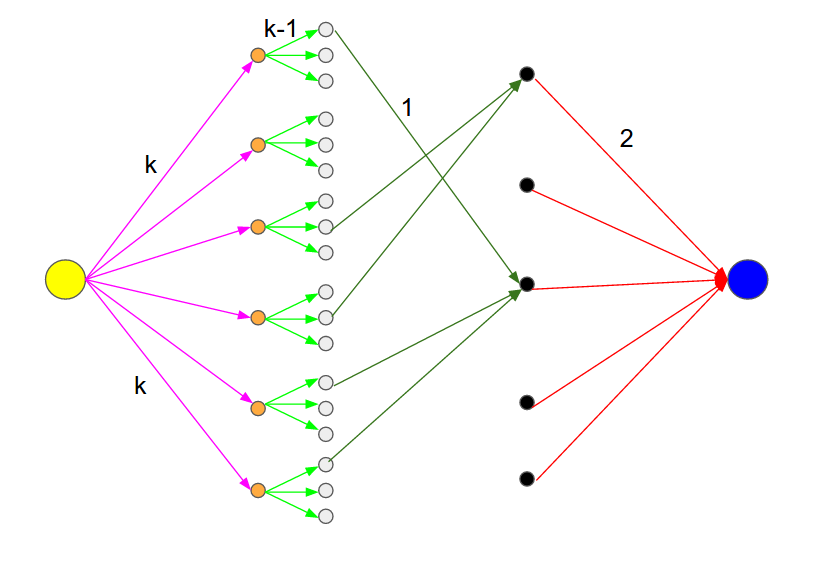
\includegraphics[width=0.5\columnwidth]{fig_dif.png}
\caption{ Edge Capacities-- Pink Edges: k, Light Green Edges: k-1, Dark Green Edges: 1, Red Edges: 2;\newline Orange Vertices: Conditions, Black Vertices: Balloons, Grey Vertices: Contractors}
\label{sim}
\end{figure}

\section{A Social Networking Problem}

\subsection{Maximisation Problem}
Let $F_i$ to be the number of friends of Person i and $F_{i,j}$ is one if i is friend of j, otherwise 0. Now, Since we want a subset X such that number of edges in X is atleast 10 times $|X|$. This translates into:
$$ \frac{\text{Number of edges in X}}{|X|} \geq 10$$
$$ \frac{1/2 \times \sum_{i \in X}F_i - \sum_{i \in X, j \in \bar{X}}F_{i,j}}{|X|} \geq 10$$
$$ \frac{\sum_{i \in X}F_i - 2 \times \sum_{i \in X, j \in \bar{X}}F_{i,j}}{|X|} \geq 20$$
Since, we have counted each edge twice, the right hand side becomes 20 instead of 10. This now becomes the following maximisation problem:
$$ q(F) = \sum_{i \in X}F_i - 2 \times \sum_{i \in X, j \in \bar{X}}F_{i,j} - 20|X| $$

\subsection{Minimisation Problem}
Using the above equation, we can transform this into a minimisation problem, so that we can solve it using min-cut theorem :
$$ q(F) =  \textbf{F} - \sum_{i \in \bar{X}}F_i - 2 \times \sum_{i \in X, j \in \bar{X}}F_{i,j} - 20|X| $$
where $\textbf{F} = \sum_{i \in V}F_i$. Thus the minimisation problem becomes:
$$ q'(F) =  \sum_{i \in \bar{X}}F_i + 2 \times \sum_{i \in X, j \in \bar{X}}F_{i,j} + 20|X| $$
\subsection{Flow Network Construction}
Consider Figure \ref{min}, which shows the flow network(directed graph) for this problem.
\begin{figure}[h!]
\centering
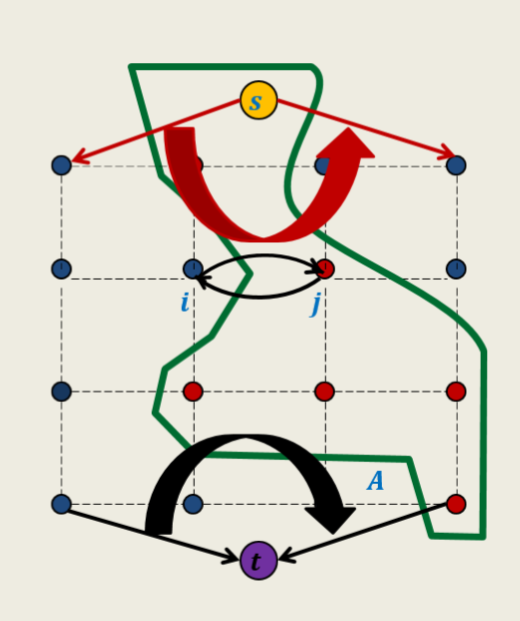
\includegraphics[width=0.5\columnwidth]{fig_minCut.png}
\caption{ Red Vertices : X , Blue Vertices : $\bar{X}$ \newline Edge Capacities: Red Edges: $F_i$ Black Edges(to sink): 20, Black Edge(between Person): 2 \newline Image Source: Lecture Slides(CS345) by Dr. Surender Baswana}
\label{min}
\end{figure}
\newline
We add a source(s) and a sink vertex (t) and assign edges and edge capacities as shown in figure. The green boundary in this graph encloses X. \\ \\
Consider the min-cut formulation of this graph:
$$ \text{Cut} = \sum_{i \in \bar{X}}c_{s,i} + \sum_{j \in X}c_{j,t} + \sum_{i \in X , j \in \bar{X}}c_{i,j}$$
$$ \text{Cut} = \sum_{i \in \bar{X}}F_i + \sum_{j \in X}20 + \sum_{i \in X , j \in \bar{X}}2$$
$$ \text{Cut} = \sum_{i \in \bar{X}}F_i +20|X| + 2 \times \sum_{i \in X, j \in \bar{X}}F_{i,j}$$
Now, FF algorithm will give a cut which minimises the above function which is precisely the minimisation function, we defined earlier.\\ \\
\textbf{Finding a Friend Group:} After finding min-cut, we will calculate (\textbf{F} - Min-Cut). If this is greater than 0, then we have the friend group and that group will be X, otherwise no such group exists.

\end{document}


